\begin{abstract}
Workforce wellbeing surveys can guide which organisations receive closer review, but collecting more responses need not resolve uncertainty about that decision. We study a fixed budget for additional measurement before allocating a fixed number of review slots. An ordinary channel may share a persistent organisation-specific offset; a more expensive validation channel measures a reference target only under an explicit validity assumption. We specialise existing Gaussian knowledge gradient to this decision and distinguish three phenomena: irreducible ranking uncertainty from unit-specific offsets, harmless shared shifts under within-group quotas, and finite-budget losses from costly or invalid validation. Controlled Gaussian experiments show both gains and reversals. A temporally separated benchmark uses 206,098 employed-adult BRFSS records from 2023 for calibration and 214,151 from 2024 for hidden-record replay across 48 areas. Under a controlled recruitment tilt and validation cost five, two-channel knowledge gradient increases severity regret from 0.1615 to 0.1857 at budget 144, despite slightly reducing estimation error. NHS aggregate data provide a separate conditional illustration, not an intervention evaluation. The contribution is an auditable decision benchmark and a characterisation of when additional measurement can fail; neither a new acquisition algorithm nor improved employee health is claimed.
\end{abstract}

\section{Introduction}
A workforce team with limited capacity may need to decide which organisations warrant a closer wellbeing review. The organisations with the lowest reported scores are not necessarily those with the greatest underlying need. Sampling noise, differential participation and changes in the measurement process can alter the list. A natural response is to collect more information before deciding. Yet an additional survey through the same recruitment channel can repeat the same distortion, while a costly independent assessment can consume the budget before resolving enough comparisons. The practical question is therefore not simply where uncertainty is largest, but which additional measurements can change a consequential decision.

The NHS provides a concrete motivation, with important limits. The annual NHS Staff Survey and quarterly staff-listening infrastructure inform workforce discussions. National Quarterly Pulse Survey guidance preserves an opportunity for all staff to respond in relevant rounds \citep{dom_nqps2023}. Targeted acquisition must therefore mean \emph{additional} follow-up on top of universal opportunity. It must not remove routine invitations from organisations judged low priority. Moreover, quarterly engagement items are not interchangeable with the annual burnout composite. Our proposed users are staff-experience leads and workforce analysts making a cross-organisation review decision; no NHS stakeholder has yet validated this workflow.

This study examines the measurement stage, not allocation of treatment or financial returns from employee wellbeing programmes. A review slot means capacity to examine a unit's situation and discuss next steps. Lower target scores indicate greater need. We minimise the difference between the average target score of the selected units and that of an oracle selection with the same capacities. This severity loss distinguishes an almost-tied substitution from overlooking a much worse unit. It also allows clear analysis of when uncertainty about a common level shift is irrelevant to a fixed within-group decision.

Our method uses established Gaussian knowledge gradient (KG) and multi-information-source optimisation (MISO), not a newly invented acquisition principle \citep{frazier2008kg,frazier2009correlated,poloczek2017miso}. The study contributes an NHS-informed decision specification, an explicit account of which uncertainty affects that specification, and a reproducible benchmark that can reject an appealing measurement policy. The benchmark separates model-generated latent truth from real recorded outcomes with controlled sampling. In the latter, calibration uses the previous year and policies cannot access the hidden current-year targets. All policies share the same inference model except designated bias-blind baselines.

Three findings challenge a blanket recommendation to validate more. First, persistent offsets matter through relevant \emph{differences}: independent unit offsets can leave selection regret even after unlimited ordinary measurement, whereas a shared within-group offset cancels from this loss. Second, myopic gain per cost does not solve the multistep budget problem. Third, on real-record replay, lower mean squared estimation error can accompany worse review selections. These findings support a limited social-impact claim: the framework can expose unjustified measurement expenditure before a field deployment. It does not establish that its recommendations improve NHS decisions or employee health.

\section{Related Work}
Gaussian KG values a measurement by the expected improvement in a subsequent decision \citep{frazier2008kg,frazier2009correlated}. MISO explicitly models discrepancies between cheaper information sources and an expensive target source \citep{poloczek2017miso}. Our independent two-dimensional unit model is a small, transparent instance of that programme. The cost-normalised rule remains myopic; nonconcavity of information value can make sequential cost ratios misleading \citep{frazier2010paradoxes}.

Optimal-subset allocation, fixed-confidence subset identification and combinatorial pure exploration have different objectives and guarantees \citep{chen2008subset,kalyanakrishnan2012pac,chen2014combinatorial}. We study expected severity regret under a fixed budget. Our boundary-directed baseline is a heuristic, not an implementation carrying a LUCB sample-complexity guarantee. Contaminated observations can prevent identification even with unlimited samples \citep{altschuler2019contaminated}. Multi-fidelity best-arm identification and recent selective proxy auditing also address cheaper biased sources \citep{poiani2024optimal,ao2026judges}. We do not claim the existence of a second channel, the Gaussian conditioning formula, or persistent-bias nonidentification as new.

AI for social impact includes resource-constrained data acquisition. \citet{dom_betti2026} study spatial mapping on a budget, and \citet{dom_goebel2026} study budgeted active learning using expert advice and episodic priors. Our distinction is between noise, persistent channel error and decision-invariant shared shifts in a review-selection task. Health-service profiling already cautions against overinterpreting ranks \citep{goldstein1996league,lin2006ranking}. Here the intervention being evaluated computationally is a \emph{measurement policy}; it is not a wellbeing intervention or a causal estimate of organisational benefit.

\section{Decision and Measurement Model}
\label{sec:model}
There are $M$ units partitioned into comparison groups $g$, with prescribed review capacities $k_g$. Let $\mathcal S=\{S:|S\cap g|=k_g\}$ and $K=\sum_g k_g$. For lower-is-worse target $\theta_i$, define
\begin{equation}
 L(S,\theta)=K^{-1}\left(\sum_{i\in S}\theta_i-\min_{A\in\mathcal S}\sum_{i\in A}\theta_i\right).
 \label{eq:lossmain}
\end{equation}
Each selected unit has equal weight. Capacities are a decision assumption, not a proven fairness criterion. Conditional on observed data, the Bayes action selects the $k_g$ smallest posterior target means in each group. Linearity of expectation establishes this decision even for dependent targets.

An ordinary measurement packet observes $Y_{iR}=\theta_i+b_i+\epsilon_{iR}$; an ideal validation packet observes $Y_{iA}=\theta_i+\epsilon_{iA}$. A persistent $b_i$ is shared across repeat packets from unit $i$. Packets have known costs $c_R,c_A$ and fresh conditional noise variance $r_{id}$. At each step an affordable unit-channel action is selected, its observation updates the posterior, and its cost is deducted. The final set is chosen when no action of that policy is affordable. Initial observations are common to every policy and excluded from the additional budget.

For acquisition, assume independent unit states and fixed hyperparameters:
\begin{equation}
 (\theta_i,b_i)\mid D\sim N\left(\begin{pmatrix}m_i\\a_i\end{pmatrix},
 P_i=\begin{pmatrix}v_i&u_i\\u_i&q_i\end{pmatrix}\right).
\end{equation}
The loading is $h_R=(1,1)^\mathsf T$ or $h_A=(1,0)^\mathsf T$. Gaussian conditioning gives
\[P_i^+=P_i-\frac{P_ih_dh_d^\mathsf TP_i}{h_d^\mathsf TP_ih_d+r_{id}}.\] The random change in target posterior mean has standard deviation
\begin{equation}
 s_{id}=\frac{|(P_ih_d)_1|}{\sqrt{h_d^\mathsf TP_ih_d+r_{id}}}.
 \label{eq:sdmain}
\end{equation}
For $a$ independent respondent draws of variance $\sigma^2$, a packet mean has noise variance $\sigma^2/a$. Persistent channel offsets do not shrink by this factor. Validation unbiasedness is an assumption, not a consequence of using different respondents.

\paragraph{Exact one-step value.}
For $0<k_g<|g|$, let $t_i$ be the $k_g$th smallest \emph{other} posterior mean and $d_i=|m_i-t_i|$. If the action changes only coordinate $i$, its expected reduction in Bayes severity risk is
\begin{equation}
 \mathrm{KG}_{id}=\frac{s_{id}\varphi(d_i/s_{id})-d_i\Phi(-d_i/s_{id})}{K},
 \label{eq:kgmain}
\end{equation}
with zero value at $s_{id}=0$ or a trivial group quota. This is the expected positive part of a normal boundary crossing. For a currently selected unit the alternative cutoff is the group's $(k_g+1)$st mean, not its $k_g$th mean. The distinction matters in implementation. Our two-channel KG policy maximises $\mathrm{KG}_{id}/c_d$ over affordable actions. The $1/K$ factor is common and can be omitted for this choice. If an observation changes multiple correlated units, the one-coordinate expression is invalid.

\paragraph{What ordinary repetition cannot learn.}
For independent priors $\theta\sim N(\mu,\tau^2)$ and $b\sim N(0,\beta^2)$, infinitely many ordinary measurements leave target variance
\begin{equation}
 V_\infty=\frac{\tau^2\beta^2}{\tau^2+\beta^2}.
\end{equation}
For two independent units and one slot, even exact observations of both $\theta_i+b_i$ leave Bayes severity regret
\begin{equation}
 R_\infty=\frac{\tau}{\sqrt\pi}\left(1-\frac{\tau}{\sqrt{\tau^2+\beta^2}}\right).
 \label{eq:floor_main}
\end{equation}
However, a positive level-variance floor does not establish selection harm. For arbitrary group constants $z_g$, every feasible set satisfies $L(S,\theta+z)=L(S,\theta)$. If the sole ordinary offset is shared within a group, exact ordinary observations identify its optimal set. A model that instead treats this shift as independent offsets can buy validation for a distinction irrelevant to the decision.

\paragraph{Validation and cost are separate assumptions.}
At the same unit and equal cost, with a nontrivial group quota, ideal validation has greater one-step value precisely when
\begin{equation}
 \frac{v_i^2}{v_i+r_{iA}}>
 \frac{(v_i+u_i)^2}{v_i+q_i+2u_i+r_{iR}}.
\end{equation}
Unequal costs require the full KG ratio; variance reduction per cost is not interchangeable with it. If validation has its own persistent offset $d$ with independent variance $\delta^2>0$, observing both channels exactly still leaves variance $(\tau^{-2}+\beta^{-2}+\delta^{-2})^{-1}$. Finally, greedy KG per cost need not optimise a fixed budget: the supplement gives a two-option Gaussian example where two cheap measurements yield expected improvement 0.3257, but one affordable expensive measurement yields 0.3804. These are reference-model statements, not guarantees for misspecified survey models. Full propositions, proofs and independent numerical checks are supplied in the supplement.

\begin{figure*}[t]
 \centering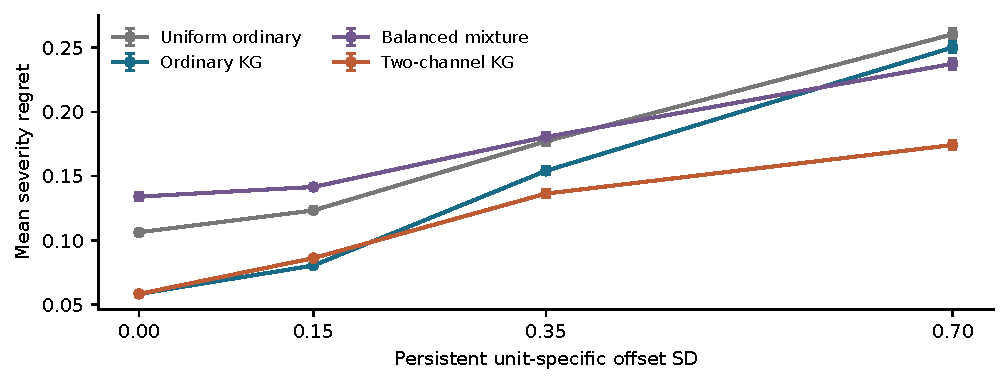
\includegraphics[width=0.85\textwidth]{figures/synthetic_bias.pdf}
 \caption{Controlled Gaussian worlds, budget 120 and validation cost 5. Lower severity regret is better. Error bars are 95\% Monte Carlo intervals from 2,000 replications per world. Policies share the same bias-aware inference model. Two-channel KG has access to more expensive information; the balanced mixture has the same channel access.}
 \label{fig:synthetic}
\end{figure*}

\section{Experimental Design}
\label{sec:experiments}
\paragraph{Policies and outcomes.}
We compare ten policies. Uniform ordinary, maximum posterior variance, a boundary heuristic and ordinary-only KG share the same bias-aware update. Bias-blind uniform and KG set the assumed offset to zero. Two-channel KG, uniform sampling over unit-channel pairs, a cost-balanced random mixture, and validation-only sampling can use validation. The balanced mixture selects validation with probability $1/(1+c_A)$ when $c_R=1$, giving equal expected channel expenditure before budget-end effects. Two-channel KG, the equal-action mixture and the balanced mixture have the same channel access; validation-only is a restricted comparator. Comparison with ordinary KG also changes the available channels. Policies consume matched per-unit, per-channel streams. We report severity regret, selected-set overlap with the oracle, target MSE, nominal 95\% interval coverage and validation spending. Coverage under misspecification is empirical, not guaranteed.

\paragraph{Controlled latent-truth experiments.}
Forty units form four groups of ten, with two review slots per group. Targets are iid $N(5,0.35^2)$; unit-specific ordinary offsets have SD $\beta\in\{0,0.15,0.35,0.70\}$. Each unit begins with 20 ordinary draws; each additional packet represents 20 draws with individual SD 2.5. Additional budgets are 40 and 120 ordinary-packet cost equivalents, with validation costs 2, 5 and 10. Each latent world has 2,000 independent replications, reused across its cost and budget settings. Seven additional worlds examine underestimated bias, overestimated bias, biased validation, heavy-tailed packet noise, unequal noise, post-initial target drift, and a shared group offset. The heavy-tail stress draws a scaled Student-$t_3$ \emph{packet mean}; it is not a sample mean of 20 individual $t_3$ variables. All stress assumptions and the complete 310 policy-setting rows are reported.

\paragraph{Real-record replay, not field validation.}
We use official CDC BRFSS public files \citep{cdc2023,cdc2024}. Eligible records report employment or self-employment and a valid number of mentally unhealthy days. The score is $(30-\mathrm{MENTHLTH})/3$, with code 88 mapped to zero days; refusal, unknown and missing values are excluded. The common cohort comprises 47 states plus DC: 206,098 eligible records in 2023 and 214,151 in 2024. The primary target is each area's \emph{unweighted complete-file eligible-respondent mean}, not population prevalence or clinical need. Nine of 48 areas are selected. These are geographical areas, not NHS trusts or hospital departments, and this outcome is not the NHS burnout composite.

Only 2023 supplies the common target-prior centre, between-area SD and within-area sampling variances. The 2024 record distribution supplies a hidden evaluation frame. Every area initially reveals 20 draws; every new packet contains 20 draws \emph{with replacement}. Sampling from the 31 outcome-frequency bins is exactly equivalent to record sampling for this single outcome. Repeated records are allowed: a packet is not 20 newly recruited people. Policies receive observations and frozen calibration, never the complete 2024 means.

Ordinary recruitment is either uniform or has probabilities proportional to $p_j\exp(\pm\kappa x_j/\sigma_{i,2023})$, with a persistent random sign per area and repetition. Values $\kappa=0.25,0.50$ are controlled mechanisms, not estimates of actual nonresponse bias. The corresponding 2023 plus/minus laws supply the working bias centre, bias variance and packet variance. This favourable knowledge of a hypothetical recruitment law is explicit. Validation is uniform except for a failure scenario with its own independent tilt of 0.25. A weighted sensitivity uses probabilities proportional to the supplied survey weights and targets the resulting \emph{weighted finite-file distribution}; it is not design-based population inference. All five scenarios use 1,000 repetitions, budgets 48 and 144, and validation costs 2, 5 and 10 for the unweighted uniform and unweighted tilt-0.50 scenarios, or cost 5 otherwise. This gives 180 policy-setting rows. The posterior is a working Gaussian approximation to bounded, asymmetric observations and a two-sign bias mechanism.

\paragraph{NHS conditional illustration.}
The 2025 release provides five-year histories for a cohort of 190 trust reporting units (189 legal entities), with 36 hypothetical within-group review slots \citep{nhs2025workbook,nhs2025technical}. A scenario analysis uses observed 2025 burnout scores, assumed $\tau=0.35$ and individual SD 2.5, and nominal respondent counts multiplied by 1 or 0.25. Neither multiplier estimates effective sample size. Candidate packets contain 20 draws, with ordinary cost one and validation cost five. We compute initial one-step gain-per-cost priorities under four assumed bias scales; no new NHS observation or intervention is generated or observed.

\paragraph{Uncertainty and audit.}
Mean intervals use MCSE across independent replications; policy differences use their paired replication differences. They quantify Monte Carlo uncertainty conditional on the specified world or fixed record frame, not uncertainty about the NHS or BRFSS populations. Cost and budget settings share worlds and are not pooled as independent evidence. Source files have retrieval timestamps and SHA-256 records. Separate code independently checks Gaussian updates, selection cutoffs, theory, record extraction, budget compliance and hidden-target exclusion. Local protocols record the design before full execution and identify later analyses; they are not external preregistrations.

\begin{table*}[t]
 \centering\small\begin{tabular}{lrrrrr}
\toprule
Policy & Unif. & T.25 & T.50 & Wgt. & V.bias \\
\midrule
Uniform ordinary & 0.1397 & 0.1813 & 0.1848 & 0.1965 & 0.1848 \\
Uniform, bias blind & 0.1397 & 0.1929 & 0.2103 & 0.2200 & 0.2093 \\
Maximum variance & 0.1343 & 0.1766 & 0.1967 & 0.2020 & 0.1950 \\
Boundary heuristic & 0.1042 & 0.1782 & 0.1885 & 0.1996 & 0.1880 \\
Ordinary KG & 0.1124 & 0.1570 & 0.1615 & 0.1773 & 0.1612 \\
Bias-blind KG & 0.1124 & 0.1894 & 0.2008 & 0.2129 & 0.1994 \\
Equal-action mixture & 0.1697 & 0.1852 & 0.1893 & 0.1990 & 0.2081 \\
Balanced mixture & 0.1558 & 0.1863 & 0.1884 & 0.2008 & 0.1998 \\
Validation only & 0.1765 & 0.1866 & 0.1899 & 0.1995 & 0.2114 \\
Two-channel KG & 0.1124 & 0.1755 & 0.1857 & 0.1959 & 0.2226 \\
\bottomrule
\end{tabular}

 \caption{Mean severity regret on real-record replay, additional budget 144, validation cost 5, 1,000 repetitions per scenario. Columns: uniform ordinary; tilt 0.25; tilt 0.50; weighted finite-frame tilt 0.50; and ordinary tilt 0.50 with validation tilt 0.25. All targets are fixed-frame recorded means. Lower is better; this table is not a population or NHS effect estimate.}
 \label{tab:replay}
\end{table*}

\begin{figure*}[t]
 \centering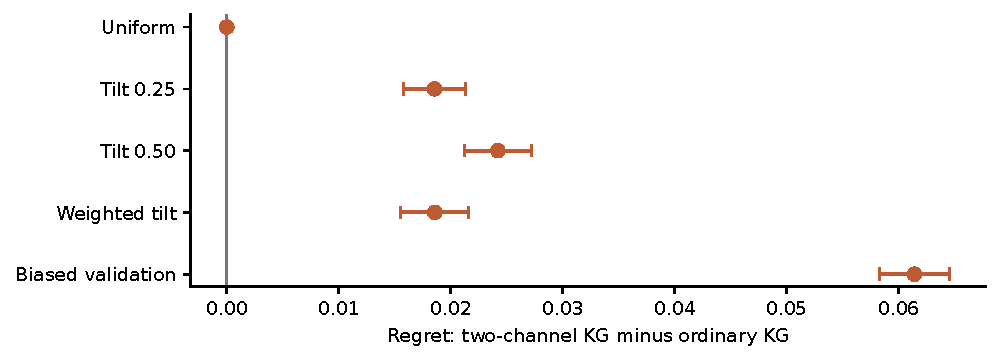
\includegraphics[width=0.85\textwidth]{figures/replay_paired.pdf}
 \caption{Paired regret differences at replay budget 144 and cost 5. Positive values mean two-channel KG is worse than ordinary KG. Intervals use paired Monte Carlo standard errors. The validation-failure condition has a separate persistent tilt; independence of its sign does not make it a valid reference channel.}
 \label{fig:paired}
\end{figure*}

\section{Results}
\paragraph{Validation helps some Gaussian worlds and harms others.}
At budget 120 and validation cost 5, increasing independent offset SD from 0.15 to 0.70 changes the comparison substantially (Figure~\ref{fig:synthetic}). At $\beta=0.15$, two-channel KG raises regret from 0.0804 to 0.0862, a paired increase of 0.0058 [0.0042, 0.0073]. At $\beta=0.35$ it reduces regret from 0.1541 to 0.1364; at $\beta=0.70$ it reduces regret from 0.2503 to 0.1743, a difference of $-0.0760$ [$-0.0803$,$-0.0716$]. With no offset it chooses only ordinary measurements and matches ordinary KG. The fraction of budget spent on validation rises from 0 at zero bias to 0.916 at $\beta=0.70$. A nonzero bias floor alone therefore does not justify an expensive finite-budget measurement policy.



\paragraph{The positive simulation result does not transfer automatically.}
Table~\ref{tab:replay} reports all ten policies at replay budget 144 and cost 5. Under tilt 0.50, ordinary KG has regret 0.1615, compared with 0.1857 for two-channel KG and 0.1884 for the balanced mixture. Two-channel KG's paired difference from ordinary KG is $+0.0242$ [0.0212, 0.0272] (Figure~\ref{fig:paired}). It spends 97.2\% of the budget on validation. It is close to uniform ordinary sampling (0.1848) and does not justify an overall claim of better decision efficiency. Its lower mean than the balanced mixture is a narrower same-action-set comparison. Under uniform sampling, the boundary heuristic has the lowest mean regret in this displayed grid; KG is not a universal winner.





\paragraph{Estimation accuracy and selection value diverge.}
In the tilt-0.50 replay, two-channel KG reduces target MSE from 0.02183 to 0.02129 while increasing severity regret. The weighted sensitivity shows the same direction: MSE falls from 0.02250 to 0.02194, but regret increases from 0.1773 to 0.1959. These descriptive comparisons concern different loss functions, not a causal decomposition of the failure. More precise levels across all units need not resolve the comparisons near a review boundary. Non-Gaussian observations, a working prior, myopia and unequal channel costs remain jointly present; the experiment does not identify a unique cause.

\paragraph{Cost, validity and model structure change the answer.}
For tilt-0.50 replay at budget 144, two-channel regret is 0.1626, 0.1857 and 0.1933 as validation cost rises from 2 to 5 to 10; ordinary KG remains at 0.1615. When validation itself has tilt 0.25, two-channel regret reaches 0.2226 versus ordinary KG's 0.1612. Gaussian stress tests also reveal reversals. With overestimated bias, regret is 0.1303 versus 0.0588; with a shared group shift it is 0.1336 versus 0.0599; after target drift it is 0.1761 versus 0.1572. Heavy-tailed packet noise, unequal noise and underestimated bias yield different comparisons, all retained in the supplement. The shared-shift result is consistent with the invariant-loss argument, while also including an intentionally misspecified independent-offset acquisition model.

\paragraph{A larger budget can reverse the replay comparison.}
After the primary analysis, we specified an exploratory extension with 500 new repetitions, the unweighted tilt-0.50 mechanism, validation cost 5, and budgets 48, 144, 480 and 1,440. All four settings were fixed before this separate run. Two-channel KG remains worse than ordinary KG at the first three budgets. At 1,440 it has regret 0.0907 versus 0.1242, a paired difference of $-0.0335$ [$-0.0379$,$-0.0291$]. It spends all additional budget on validation at the two largest budgets. Thus the last comparison concerns adaptive selection of validation units, not successful balancing of channels. Uniform validation has regret 0.1229 at the same expenditure of 1,440. The supplement retains the whole extension and its post-primary status; it does not establish an NHS spending threshold.

\paragraph{NHS sensitivity.}
The historical cohort has median nominal burnout count 3,140.5. With nominal counts treated as effective and assumed $\beta=0$, the 20 units with greatest initial measurement value per cost all prefer ordinary packets. At assumed $\beta=0.15$, all 20 prefer validation. With the count multiplier reduced to 0.25, only 15 prefer validation at that bias scale. This change is a sensitivity result, not an empirical estimate of nonresponse bias or a recommendation to contact those units. It demonstrates why precision and channel-validity assumptions must accompany any operational list.

\section{Social-Impact Pathway and Limitations}
The intended human decision is whether to spend an additional information budget before allocating scarce review capacity. The algorithm allocates a given budget among permitted measurements; it does not optimise whether to collect any new data or implement a value-based stopping rule. A usable interface would show the provisional review set, its sensitivity to precision and bias assumptions, the reason an additional observation could alter the set, expected cost and the conditions under which that channel is valid. Routine participation opportunities remain intact. Requests for immediate staff support must never wait for an acquisition algorithm to resolve a ranking.

The computational loss is deliberately limited. It values selected units equally, not employees equally, does not measure treatment benefit, and may miss a vulnerable subgroup hidden inside an organisational average. Within-group quotas preserve comparability only by assumption; they do not establish equitable access. Respondent burden, invitation effort, nonresponse, confidentiality and analysis time are absent from the packet-cost model. Twenty completed draws are purchasable by construction in the simulator, not guaranteed through real recruitment. NHS guidance emphasises connecting listening to visible action \citep{dom_listeningwell2023}; an algorithm that generates more questionnaires without follow-through could impose costs without benefit.

Before operational use, the reference measurement must be defined and tested for the same construct and population. Independent respondents alone are insufficient. A stakeholder study would need to verify the proposed review decision, acceptable delay, cost accounting and overrides. A prospective evaluation could compare equal-budget measurement policies using a prespecified independent reference and assess decision changes, burden, participation and subgroup coverage; downstream health effects would require a separate appropriate causal design. These studies have not occurred. BRFSS replay provides individual-record evidence for controlled measurement decisions, not validation of an NHS deployment.

Our theoretical formulas assume fixed Gaussian hyperparameters and independent unit states for one-coordinate acquisition. Real records violate the exact reference model; the deliberately favourable 2023 bias calibration is unavailable without extra knowledge in practice. The cohort and one held-out target year do not establish broad transfer. Replays sample with replacement from complete-case frames and exclude people with missing outcomes; weighted replay still does not resolve survey nonresponse or complex-design inference. Monte Carlo intervals do not cover these sources of uncertainty. Existing KG and MISO ideas, rather than algorithmic novelty, anchor the contribution. The resulting evidence supports targeted scrutiny of measurement policies: repeating data can preserve bias, validation can be too costly or invalid, and reducing uncertainty is valuable only relative to the actual decision.
